\documentclass{article}
\usepackage[utf8]{inputenc}
\usepackage{amsmath,amssymb,amsthm,tabu,enumerate,tikz}
\usepackage[margin=1in]{geometry}
\usepackage{verbatim} % Allows Multi-line comments 
\usepackage{multicol}
\usetikzlibrary{automata,positioning}
\newcommand{\encode}[1]{\langle #1 \rangle}
\usepackage[parfill]{parskip}
\usepackage[hyphens]{url}
\usepackage{titlesec}
\usepackage{indentfirst}
\usepackage{soul}


\usepackage{graphicx}
\usepackage{hyperref}
\graphicspath{ {images/} }

\titlespacing\section{0pt}{12pt plus 4pt minus 2pt}{0pt plus 2pt minus 2pt}
\titlespacing\subsection{0pt}{12pt plus 4pt minus 2pt}{0pt plus 2pt minus 2pt}
\titlespacing\subsubsection{0pt}{12pt plus 4pt minus 2pt}{0pt plus 2pt minus 2pt}

\title{FRC Java Startup Guide}
\author{dcobbley }
\date{October 2016}

\begin{document}

\maketitle

\section{Introduction}
Follow these steps carefully to setup the java programming environment for FRC robotics. These instructions were developed for windows but should easily translate to Linux.

*Note: Don’t confuse the preference menu with the properties menu.

\begin{enumerate}
    \item To start, follow the instructions found here:
    
    \url{https://wpilib.screenstepslive.com/s/4485/m/13809/l/599681-installing-eclipse-c-java}
    \begin{enumerate}[(a)]
        \item Download JDK
        
        \url{http://www.oracle.com/technetwork/java/javase/downloads/index.html}

    
    \href{http://www.oracle.com/technetwork/java/javase/downloads/index.html}{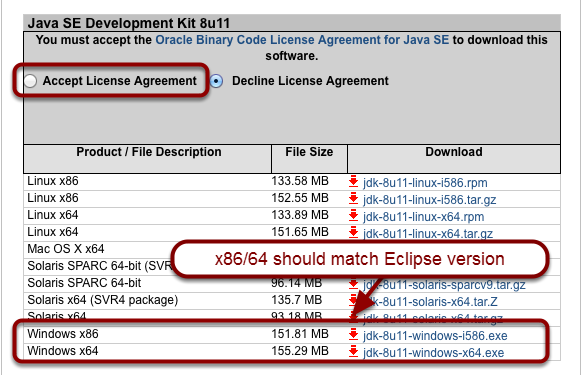
\includegraphics[scale=.5]{1a.png}}
    
    
        \item Install Eclipse - Newest is now Neon. Select the “Download Pacakges” option under the large orange button:
        
        \url{http://www.eclipse.org/downloads/}
        
        \href{http://www.eclipse.org/downloads/}{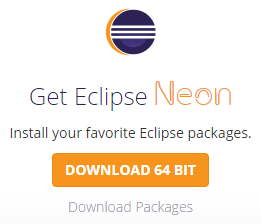
\includegraphics[scale=.7]{1b.png}}
        
        Extract the contents of the zip file by right-clicking on the .zip file in a windows explorer window and selecting "Extract All..." and taking the default for the location to extract it.
        
        Move the extracted folder to Program Files or some other convenient location from which to easily run it. Within the eclipse folder you'll see the file "eclipse.exe". You can right-click on "eclipse.exe" and select "Pin to start menu" to make it easier to run eclipse without having to find the installation location.
        
    \end{enumerate}
    
    \item Setup JDK
    
    \begin{enumerate}[(a)]
        \item Navigate to Windows $\rightarrow$ preferences
        
        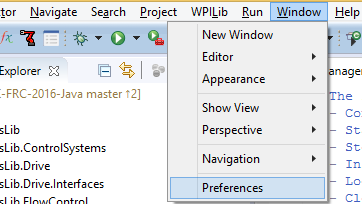
\includegraphics{2a.png}
        
        \item Then Java $\rightarrow$ Installed JREs
        
        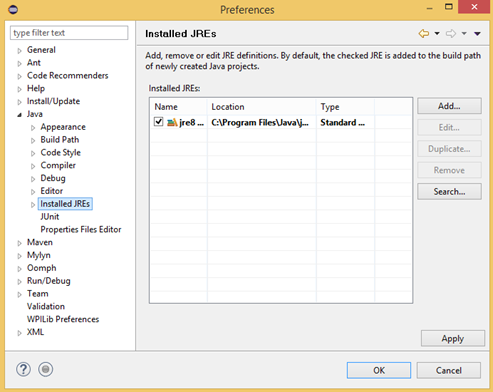
\includegraphics{2b.png}
        
        Notice under name that it says jre8 and location will most likely be $\backslash$Java$\backslash$JRE8...
        \pagebreak
        \item Double click on the location of jre8, you should see:
        
        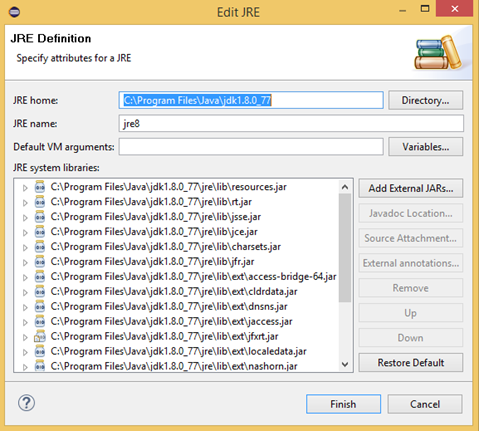
\includegraphics{2c.png}

        \item Go ahead and change the location of JRE home to the path for your JDK. For some reason we have to lie to Java, we want to use the developement kit, not the runtime environment. Click Finish.
        
        \item Set a few extra preferences, starting with auto save: Window $\rightarrow$ Preferences $\rightarrow$ General $\rightarrow$ Workspace $\rightarrow$ Check Save automatically before build $\rightarrow$ OK	
        
        
        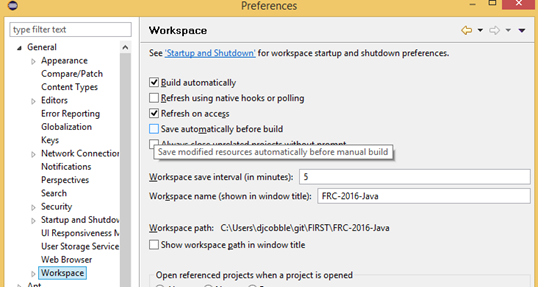
\includegraphics{2f.png}
        
        \item While you’re still in the preferences, go to Install/Update: check Automatically find new updates and notify me. Making sure this is run every time Eclipse is started.
        
        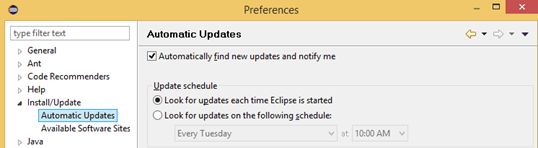
\includegraphics{2g.png}
        
        \end{enumerate}
        \vspace{5mm}
        \item Next we will add the WPI library. Navigate to Help$\rightarrow$Install New Software:
        
        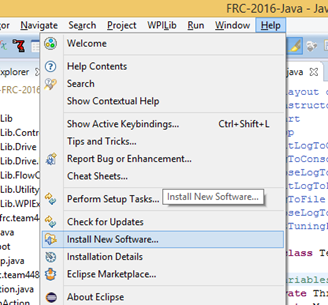
\includegraphics[scale=.85]{2h.png}
        
        \item Click Add, and enter Name: “FRC Plugins” \& enter its Location:
        
        \url{http://first.wpi.edu/FRC/roborio/release/eclipse/}

        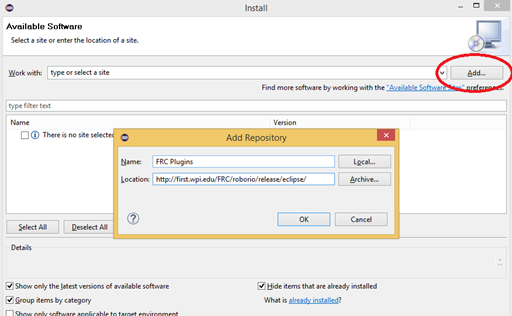
\includegraphics[scale=.95]{2i.png}
        
        \item Select Robot Java Development, we do not need C++
        
        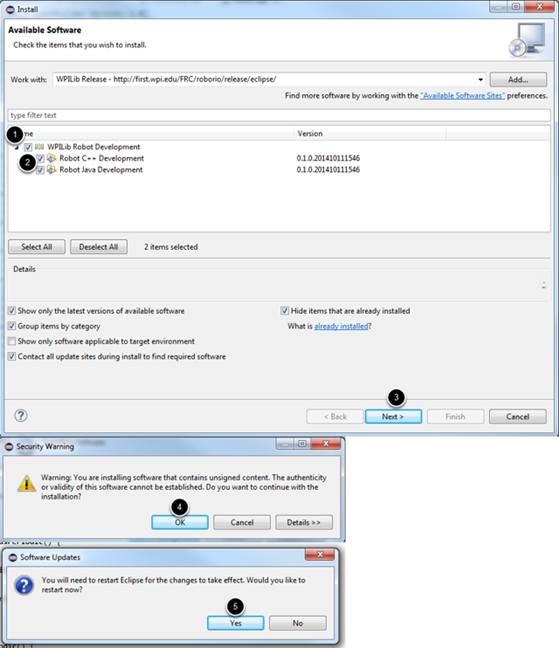
\includegraphics[scale=.97]{2j.png}
        
        \item Finish up by checking for updates to the plugins: Help $\rightarrow$ Check For Updates

        \item Once you have downloaded the Navex, you can continue configuring Eclipse.
        \begin{enumerate}[(a)]
            \item Config settings (follow install instructions)
            \item Install dev plugins
        \end{enumerate}
        
    
    
    \item Download navx library from here: 
    \url{http://www.pdocs.kauailabs.com/navx-mxp/software/roborio-libraries/java/}
        \begin{enumerate}[(a)]
        \item Run setup.exe
        \item Configure eclipse for navx
        \url{http://www.pdocs.kauailabs.com/navx-mxp/software/roborio-libraries/java/}
        \end{enumerate}


    \item \st{Download a git plugin for eclipse}
    
    \item Sync to team repo
    
    import $\rightarrow$ ProjectsFromGit  $\rightarrow$  CloneURL

    \item Point to downloaded libraries
        \begin{enumerate}[(a)]
        \item Right click on Preferences $\rightarrow$ Java $\rightarrow$  Build Path  $\rightarrow$  Class Path Variables $\rightarrow$ edit $\rightarrow$ Variable $\rightarrow$ new -- Enter \textless Same Name\textgreater -- Folder 
        \item Navex variable to C:User$\backslash$ \textless user\textgreater navex
        \item Same for WPI lib
        \end{enumerate}
        
    \item Add wpilib.sources
    
    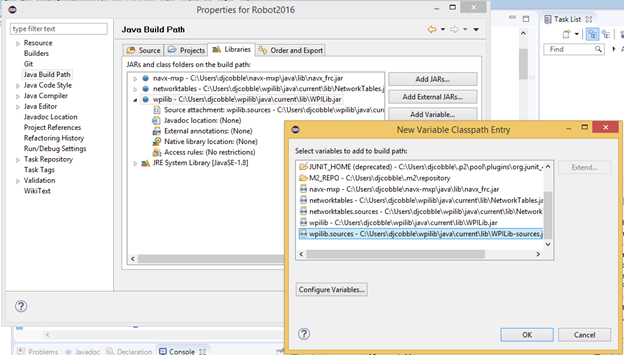
\includegraphics{7a.png}

\end{enumerate}

\section{Extras}
ANT errors:
\url{http://stackoverflow.com/questions/15098258/ant-java-home-does-not-point-to-the-jdk-but-it-does}

Set Team Number

Lots of information here:
\url{https://wpilib.screenstepslive.com/s/4485/m/13809}

Helpful information here as well:
\url{https://wpilib.screenstepslive.com/s/4485/m/13809/l/242586-building-and-downloading-a-robot-project-to-the-roborio}
\end{document}
